\section{Early detection and intervention in type 2 diabetes} \label{intro:screening}
%\paragraph{Secondary prevention of T2D is effective} 
Studies have convincingly shown that early detection and treatment of T2D can prevent or delay complications of the disease \citep{haffner1990cardiovascular,engelgau2000screening, diabetes2002reduction, genuth2003implications, holman200810, gaede2008effect, echouffo2011screening}. Additionally, treatment of early-stage T2D is often relatively simple and cheap (e.g. lifestyle changes, often specifically targetted towards weight loss) compared to the treatment of progressed T2D, which typically involves strict pharmacological therapy along with the treatment of potential complications \citep{pan1997effects,tuomilehto2001prevention,diabetes2002reduction,zammitt2005hypoglycemia}, indicating the value of early detection. The successive steps of a typical diagnostic process are shown in Figure~\ref{intro:screening-funnel}.

\begin{figure}[!h]
  \centering
  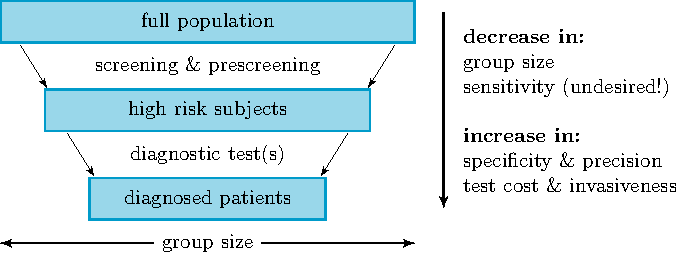
\includegraphics[width=\textwidth]{screening-funnel.pdf}
  \caption{The stages of the medical diagnostic process: screening is used to identify patients at high risk, which are then forwarded to diagnostic tests. The cost and invasiveness of tests increase as patients move down the funnel, hence each step aims to remove negatives while retaining positives. } 
  \label{intro:screening-funnel}
\end{figure}

%\paragraph{T2D is often diagnosed very late} 
Despite its widely-recognized importance, early detection of T2D proves to be problematic, as one fourth up to one third of T2D patients are estimated to be undiagnosed in developed countries \citep{diabetesliga, beagley2014global, american2014standards} and typically years pass between the onset of T2D and its clinical diagnosis \citep{harris1992onset}. In fact, the clinical diagnosis of T2D often follows signs of serious complications, which have developed during the latent stage of the disease \citep{rajala1998prevalence,harris2000early, hu2002elevated, american2014standards}. 

%\paragraph{Barriers for early detection of T2D} 
Diagnostic inertia for T2D arises in several ways. First, the disease may remain asymptomatic for many years \citep{alberti1998report}, during which unmanaged hyperglycemia may induce serious and irreversible development of micro -and macrovascular complications \citep{fowler2008microvascular, beagley2014global}. 
%Second, healthcare information related to a specific patient is often fragmented across databases of individual caregivers and other medical stakeholders, potentially causing situations in which various subtle symptoms of diabetes are presented to multiple caregivers, but the diagnosis remains elusive because each individual caregiver cannot see the big picture. 
Second, health and healthcare information related to a specific patient is often fragmented across databases of individual caregivers and other medical stakeholders. This can induce situations in which various subtle symptoms of diabetes are presented to multiple caregivers, but the diagnosis remains elusive because each individual caregiver receives too little information to spot the slumbering slayer.
Finally, universal screening for T2D is cost-prohibitive \citep{wareham2001should, engelgau2000screening}, though many organizations advise opportunistic screening of high-risk subgroups \citep{world1994prevention, alberti1998report, engelgau2000screening,american2014standards}.

Certain metabolic abnormalities typically precede T2D and can therefore be used as proverbial miners' canaries by screening approaches, specifically:
%Type 2 diabetes is typically preceded by the following metabolic abnormalities:
\begin{itemize}
\item \emph{Impaired fasting glucose (IFG)}, also known as prediabetes, is a condition in which fasting blood glucose levels are consistently higher than normal, but not high enough to warrant a diabetes diagnosis. Some patients with IFG can also be diagnosed with impaired glucose tolerance.
\item \emph{Impaired glucose tolerance (IGT)} is a prediabetic state of hyperglycemia which may precede T2D by many years. IGT is detected as an abnormal response to the oral glucose tolerance test (OGTT, cfr. Section~\ref{diagnosis-diabetes}). Specifically, patients with IGT exhibit raised glucose levels after 2 hours compared to healthy people, but not high enough to qualify for T2D. Patients with IGT present a higher risk for diabetes than patients with IFG. Approximately $40\%$ of subjects with IGT progress to diabetes over the next decade \citep{zimmet2001global}. Additionally, subjects with IGT have heightened risk of macrovascular disease compared to subjects with IFG \citep{tominaga1999impaired, unwin2002impaired}.
\end{itemize}
Both IFG and IGT are associated with insulin resistance and increased risk of diabetes and cardiovascular pathologies, with IGT being more strongly associated with cardiovascular outcomes \citep{unwin2002impaired}. Although the transition of IFG and/or IGT to diabetes may take many years, the majority of individuals with these pre-diabetic states eventually develop diabetes \cite{tuomilehto2001prevention,diabetes2002reduction,nathan2007impaired}. Additionally, the risk of complications is known to commence many years before the onset of clinical diabetes \cite{haffner1990cardiovascular,zimmet2001global}.

In the remainder of this Section we will discuss current diagnostic tests, existing screening programmes and the Belgian situation and recommendations.


\subsection{Diagnosis of diabetes} \label{diagnosis-diabetes}
The gold standard to diagnose hyperglycemia is the oral glucose-tolerance test (OGTT), which determines how quickly glucose is cleared from the blood \citep{alberti1998definition, world2006definition}. In this test, patients are administered glucose after fasting for 12 hours and afterwards the patient's blood glucose levels are measured, sometimes at multiple intervals, but typically after 2 hours \citep{diabetesliga}.

Type 1 diabetes has a sufficiently pronounced clinical onset characterized by acute, extreme elevations in glucose concentrations combined with symptoms which make its diagnosis fairly unambiguous and typically timely \citep{international2009international}. Type 2 diabetes, however, has a more gradual onset making its diagnosis less straightforward and causing the diagnostic criteria to be debated regularly \citep{world2006definition, international2009international}.  The diagnostic criteria as currently recommended by the WHO are listed in Table~\ref{intro:who-diagnosis}.

The OGTT was widely agreed upon as diagnostic test, though in 2003 the American Diabetes Association (ADA) modified its recommendations in favor of using fasting plasma glucose to diagnose asymptomatic T2D \citep{world2006definition}. More recently, the use of the A1C assays for diagnosis was considered, though current point-of-care A1C assays were considered insufficiently accurate \citep{international2009international}.

\begin{table}[!h]
\colorbox{gray!20!white}{\parbox{\textwidth}{
\begin{itemize}
\item impaired fasting glucose (IFG):
\begin{itemize}
\item fasting plasma glucose $\geq 6.1$ and $< 7.0$ mmol/l, and
\item 2-hour plasma glucose $< 7.8$ mmol/l (if measured).
\end{itemize}
\item impaired glucose tolerance (IGT):
\begin{itemize}
\item fasting plasma glucose $< 7.0$ mmol/l, and
\item 2-hour plasma glucose $\geq 7.8$ and $< 11.1$ mmol/l.
\end{itemize}
\item diabetes:
\begin{itemize}
\item fasting plasma glucose $\geq 7.0$ mmol/l, or
\item 2-hour plasma glucose $\geq 11.1$ mmol/l.
\end{itemize}
\end{itemize}
}}
\caption{Diagnostic criteria for diabetes and related metabolic abnormalities as recommended by the WHO \citep{world2006definition}.} \label{intro:who-diagnosis}
\end{table}

\subsection{Existing screening and prescreening approaches} \label{intro:screening-existing}
The clinical inertia in diagnosing type 2 diabetes is being tackled by a wide variety of screening and prescreening approaches, which commonly rely on information that is already available or relatively easy to obtain. The main method to implement such screening methods is via questionnaires, possibly paired with clinical information such as parameters recorded in patients' electronic health records or by general practioners. 

The Cambridge Risk Score (CRS) was developed to assess the probability of undiagnosed T2D based on data that is routinely available in primary care records, including age, sex, medication use, family history of diabetes, BMI and smoking status \citep{griffin2000diabetes}, The CRS and comparable scores have been shown to be useful on multiple occasions \citep{baan1999performance,griffin2000diabetes, park2002performance, spijkerman2004performance}. 
The FINDRISC score is based on a 10-year follow-up using age, BMI, waist circumference, history of antihypertensive drugs and high blood glucose, physical activity and diet and is used to predict drug-treated diabetes \citep{lindstrom2003diabetes}. The strongest reported predictors in this study were BMI, waist circumference, history of high blood glucose and physical activity. Gl{\"u}mer et al. \citep{glumer2004danish} developed a risk score based on age, sex, BMI, known hypertension, physical activity and family history of diabetes. The German diabetes risk score is based on age, waist circumference, height, history of hypertension, physical activity, smoking, and diet \citep{schulze2007accurate}.
More complex risk scores include various clinical parameters \citep{heikes2008diabetes, stern2002identification, mcneely2003comparison}.



%Simple questionnaires using only basic information can be a powerful tool to detect people that are at risk for diabetes, as proven in other countries [14–17].
%[14] Jaana Lindstr ̈om and Jaakko Tuomilehto. The diabetes risk score: a practical tool to predict type 2 diabetes risk. Diabetes Care, 26:725–731, 2003.
%[15] Charlotte Glumer, Bendix Carstensen, Annelli Sandbæk, Torsten Lauritzen, Torben Jørgensen, and Knut Borch-Johnsen. A danish diabetes risk score for targeted screening: the inter99 study. Diabetes Care, 27:727–733, 2004.
%[16] Caroline A. Baan, Johannes B. Ruige, Ronald P. Stolk, Jacqueline C.M. Witteman, Jacqueline M. Dekker, Robert J. Heine, and Edith J.M. Feskens. Performance of a predictive model to identify undiagnosed diabetes in a health care setting. Diabetes Care, 22:213–219, 1999.
%[17] Griffin SJ, Little PS, Hales CN, Kinmonth AL, and Wareham NJ. Diabetes risk score: towards earlier detection of type 2 diabetes in general practice. Diabetes Metab Res Rev, 16:164–171, 2000

%%%%%%%%%%%%%%%%%%%%%%%%%%%%%%%%%%%%%%%%%%%%%%%%%5
%
%		IN BELGIUM
%
%%%%%%%%%%%%%%%%%%%%%%%%%%%%%%%%%%%%%%%%%%%%%%%%%5


\subsection{Situation in Belgium} \label{intro:screening-belgium}
The IDF estimates over 170,000 undiagnosed diabetes patients in Belgium \citep{IDFatlas}. The Diabetes Liga estimates that currently one out of three T2D patients are undiagnosed, that one out of ten Belgians will have type 2 diabetes in 2030 and that $8\%$ and $6.5\%$ of the Belgian population currently has diabetes or prediabetes, respectively \citep{diabetesliga}. Domus Medica\footnote{A non-profit organization of general practionners that focuses on preventive medicine.} advises against population-wide screening, though it recommends case finding in high-risk subpopulations \citep{wens2005aanbeveling}, for instance via the risk factors listed in Table~\ref{intro:diabetes-liga-risk}.
\begin{table}[!h]
\colorbox{gray!20!white}{\parbox{\textwidth}{
\begin{itemize}
\item Persons of 18--45 years of age that meet one of the following conditions:
\begin{itemize}
\item prior history of gestational diabetes
\item prior history of stress-induced hyperglycemia
\end{itemize}
\item or two of the following conditions:
\begin{itemize}
\item prior history of giving birth to a baby of over 4.5 kg
\item diabetes in first-line relatives (mother, father, sister, brother)
\item BMI $\geq$ 25 kg/m$^2$
\item waist circumference $>88$ cm (for women) or $>102$ cm (for men)
\item treated for high blood pressure or with corticoids
\end{itemize}
\item Persons of 45--64 years of age that meet one of the conditions listed above.
\item Persons above 64 years old, regardless of additional risk factors.
\end{itemize}
}}
\caption{High-risk subpopulations according to the Diabetes Liga \citep{diabetesliga}.} \label{intro:diabetes-liga-risk}
\end{table}

The Belgian Scientific Institute of Public Health (WIV-ISP) reports that screening efforts are increasing in Belgium, but also indicates a need for risk stratification that goes beyond selecting all patients above a given age \citep{wivisp}.




% The onset of type 2 diabetes may occur up to 7 years before clinical diagnosis
% Harris MI, Klein R, Welborn TA, Knuiman MW. Onset of NIDDM occurs at least 4–7 years before clinical diagnosis. Diabetes Care 1992; 15:815–819. Cowie CC, Rus

% see also http://www.nature.com/nature/journal/v414/n6865/full/414782a.html

%The worldwide epidemiology of type 2 diabetes mellitus—present and future perspectives Lei Chen, Dianna J. Magliano and Paul Z. Zimmet
% The causes of the epidemic of T2DM are embedded in a very complex group of genetic and epigenetic systems interacting within an equally complex societal framework that determines behavior and environmental influences. This complexity is reflected in the diverse topics discussed in this Review. In the past few years considerable emphasis has been placed on the effect of the intrauterine environment in the epidemic of T2DM, particularly in the early onset of T2DM and obesity. Prevention of T2DM is a ‘whole-of-life’ task and requires an integrated approach operating from the origin of the disease.

% Full Accounting of Diabetes and Pre-Diabetes in the U.S. Population in 1988 –1994 and 2005–2006
% U.S. was 9.3%, of which 30% was undiagnosed based on fasting plasma glucos

% http://www.diabetesresearchclinicalpractice.com/article/S0168-8227(13)00384-7/abstract
% Globally, 45.8%, or 174.8 million of all diabetes cases in adults are estimated to be undiagnosed, ranging from 24.1% to 75.1% across data regions. An estimated 83.8% of all cases of UDM are in low- and middle-income countries. At a country level, Pacific Island nations have the highest prevalence of UDM.

% http://www.bettycjung.net/Pdfs/Alberti.pdf

% http://europepmc.org/abstract/med/18350480

% http://www.researchgate.net/profile/Leonor_Guariguata/publication/259153000_Global_estimates_of_undiagnosed_diabetes_in_adults_for_2013_for_the_IDF_Diabetes_Atlas/links/54f583fc0cf2ba61506653fb.pdf








%uit \citep{american2014standards}:
%Mass screening of asymptomatic individuals has not effectively identified those with prediabetes or diabetes, and rigorous clinical trials to provide such proof are unlikely to occur. In a large randomized controlled trial (RCT) in Europe, general practice patients between the ages of 40–69 years were screened for diabetes, then randomized by practice to routine diabetes care or intensive treatment of multiple risk factors. After 5.3 years of follow-up, CVD risk factors were modestly but significantly improved with intensive treatment. Incidence of first CVD event and mortality rates were not significantly different between groups \citep{griffin2011effect}. This study would seem to add support for early treatment of screen-detected diabetes, as risk factor control was excellent even in the routine treatment arm and both groups had lower event rates than predicted. The absence of a control unscreened arm limits the ability to definitely prove that screening impacts outcomes. Mathematical modeling studies suggest that screening, independent of risk factors, beginning at age 30 or 45 years is highly cost-effective \$11,000 per quality-adjusted life-year gained) \citep{kahn2010age}.


